% Created by tikzDevice version 0.12.3 on 2020-06-02 20:31:28
% !TEX encoding = UTF-8 Unicode
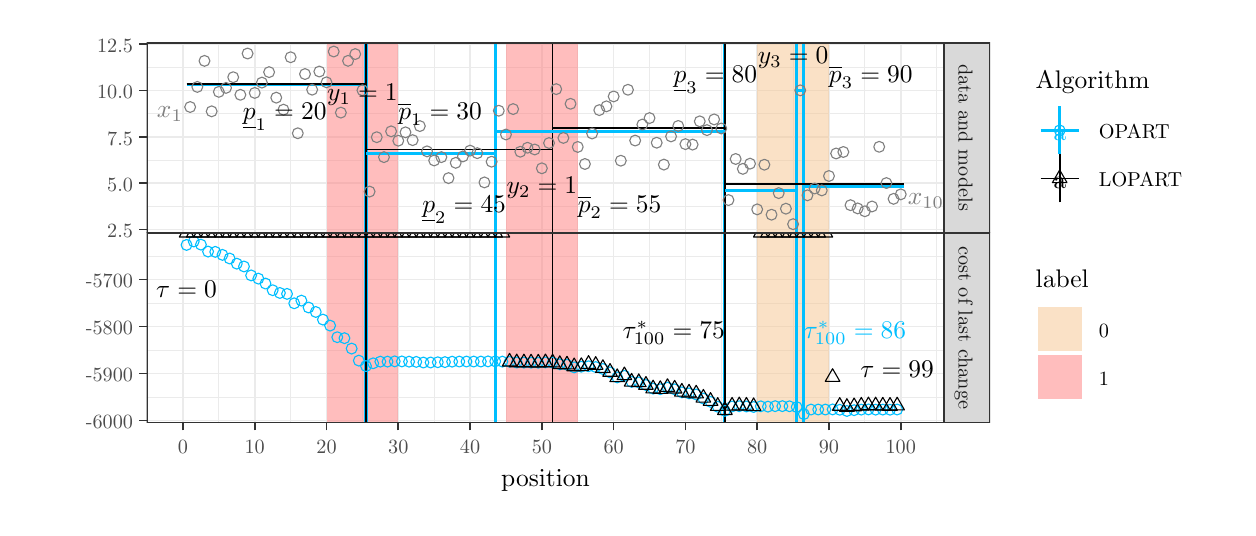
\begin{tikzpicture}[x=1pt,y=1pt]
\definecolor{fillColor}{RGB}{255,255,255}
\path[use as bounding box,fill=fillColor,fill opacity=0.00] (0,0) rectangle (433.62,173.45);
\begin{scope}
\path[clip] (  0.00,  0.00) rectangle (433.62,173.45);
\definecolor{drawColor}{RGB}{255,255,255}
\definecolor{fillColor}{RGB}{255,255,255}

\path[draw=drawColor,line width= 0.6pt,line join=round,line cap=round,fill=fillColor] (  0.00,  0.00) rectangle (433.62,173.45);
\end{scope}
\begin{scope}
\path[clip] ( 43.01, 99.32) rectangle (331.18,167.95);
\definecolor{fillColor}{RGB}{255,255,255}

\path[fill=fillColor] ( 43.01, 99.32) rectangle (331.18,167.95);
\definecolor{drawColor}{gray}{0.92}

\path[draw=drawColor,line width= 0.3pt,line join=round] ( 43.01,108.86) --
	(331.18,108.86);

\path[draw=drawColor,line width= 0.3pt,line join=round] ( 43.01,125.64) --
	(331.18,125.64);

\path[draw=drawColor,line width= 0.3pt,line join=round] ( 43.01,142.41) --
	(331.18,142.41);

\path[draw=drawColor,line width= 0.3pt,line join=round] ( 43.01,159.19) --
	(331.18,159.19);

\path[draw=drawColor,line width= 0.3pt,line join=round] ( 43.14, 99.32) --
	( 43.14,167.95);

\path[draw=drawColor,line width= 0.3pt,line join=round] ( 69.08, 99.32) --
	( 69.08,167.95);

\path[draw=drawColor,line width= 0.3pt,line join=round] ( 95.02, 99.32) --
	( 95.02,167.95);

\path[draw=drawColor,line width= 0.3pt,line join=round] (120.96, 99.32) --
	(120.96,167.95);

\path[draw=drawColor,line width= 0.3pt,line join=round] (146.89, 99.32) --
	(146.89,167.95);

\path[draw=drawColor,line width= 0.3pt,line join=round] (172.83, 99.32) --
	(172.83,167.95);

\path[draw=drawColor,line width= 0.3pt,line join=round] (198.77, 99.32) --
	(198.77,167.95);

\path[draw=drawColor,line width= 0.3pt,line join=round] (224.71, 99.32) --
	(224.71,167.95);

\path[draw=drawColor,line width= 0.3pt,line join=round] (250.64, 99.32) --
	(250.64,167.95);

\path[draw=drawColor,line width= 0.3pt,line join=round] (276.58, 99.32) --
	(276.58,167.95);

\path[draw=drawColor,line width= 0.3pt,line join=round] (302.52, 99.32) --
	(302.52,167.95);

\path[draw=drawColor,line width= 0.3pt,line join=round] (328.45, 99.32) --
	(328.45,167.95);

\path[draw=drawColor,line width= 0.6pt,line join=round] ( 43.01,100.48) --
	(331.18,100.48);

\path[draw=drawColor,line width= 0.6pt,line join=round] ( 43.01,117.25) --
	(331.18,117.25);

\path[draw=drawColor,line width= 0.6pt,line join=round] ( 43.01,134.03) --
	(331.18,134.03);

\path[draw=drawColor,line width= 0.6pt,line join=round] ( 43.01,150.80) --
	(331.18,150.80);

\path[draw=drawColor,line width= 0.6pt,line join=round] ( 43.01,167.57) --
	(331.18,167.57);

\path[draw=drawColor,line width= 0.6pt,line join=round] ( 56.11, 99.32) --
	( 56.11,167.95);

\path[draw=drawColor,line width= 0.6pt,line join=round] ( 82.05, 99.32) --
	( 82.05,167.95);

\path[draw=drawColor,line width= 0.6pt,line join=round] (107.99, 99.32) --
	(107.99,167.95);

\path[draw=drawColor,line width= 0.6pt,line join=round] (133.92, 99.32) --
	(133.92,167.95);

\path[draw=drawColor,line width= 0.6pt,line join=round] (159.86, 99.32) --
	(159.86,167.95);

\path[draw=drawColor,line width= 0.6pt,line join=round] (185.80, 99.32) --
	(185.80,167.95);

\path[draw=drawColor,line width= 0.6pt,line join=round] (211.74, 99.32) --
	(211.74,167.95);

\path[draw=drawColor,line width= 0.6pt,line join=round] (237.67, 99.32) --
	(237.67,167.95);

\path[draw=drawColor,line width= 0.6pt,line join=round] (263.61, 99.32) --
	(263.61,167.95);

\path[draw=drawColor,line width= 0.6pt,line join=round] (289.55, 99.32) --
	(289.55,167.95);

\path[draw=drawColor,line width= 0.6pt,line join=round] (315.49, 99.32) --
	(315.49,167.95);
\definecolor{drawColor}{gray}{0.50}

\node[text=drawColor,anchor=base east,inner sep=0pt, outer sep=0pt, scale=  0.92] at ( 56.11,140.98) {$x_{1}$};

\node[text=drawColor,anchor=base west,inner sep=0pt, outer sep=0pt, scale=  0.92] at (318.08,109.42) {$x_{100}$};
\definecolor{fillColor}{RGB}{255,125,125}

\path[fill=fillColor,fill opacity=0.50] (107.99, 99.32) rectangle (133.92,167.95);

\path[fill=fillColor,fill opacity=0.50] (172.83, 99.32) rectangle (198.77,167.95);
\definecolor{fillColor}{RGB}{246,196,143}

\path[fill=fillColor,fill opacity=0.50] (263.61, 99.32) rectangle (289.55,167.95);
\definecolor{drawColor}{RGB}{0,191,255}

\path[draw=drawColor,line width= 1.1pt,line join=round] (122.25, 99.32) -- (122.25,167.95);

\path[draw=drawColor,line width= 1.1pt,line join=round] (168.94, 99.32) -- (168.94,167.95);

\path[draw=drawColor,line width= 1.1pt,line join=round] (251.94, 99.32) -- (251.94,167.95);

\path[draw=drawColor,line width= 1.1pt,line join=round] (277.88, 99.32) -- (277.88,167.95);

\path[draw=drawColor,line width= 1.1pt,line join=round] (280.47, 99.32) -- (280.47,167.95);
\definecolor{drawColor}{RGB}{0,0,0}

\path[draw=drawColor,line width= 0.6pt,line join=round] (122.25, 99.32) -- (122.25,167.95);

\path[draw=drawColor,line width= 0.6pt,line join=round] (189.69, 99.32) -- (189.69,167.95);

\path[draw=drawColor,line width= 0.6pt,line join=round] (251.94, 99.32) -- (251.94,167.95);
\definecolor{drawColor}{RGB}{0,191,255}

\path[draw=drawColor,line width= 1.1pt,line join=round] ( 57.41,153.04) -- (122.25,153.04);

\path[draw=drawColor,line width= 1.1pt,line join=round] (122.25,127.83) -- (168.94,127.83);

\path[draw=drawColor,line width= 1.1pt,line join=round] (168.94,136.09) -- (251.94,136.09);

\path[draw=drawColor,line width= 1.1pt,line join=round] (251.94,114.57) -- (277.88,114.57);

\path[draw=drawColor,line width= 1.1pt,line join=round] (277.88,150.80) -- (280.47,150.80);

\path[draw=drawColor,line width= 1.1pt,line join=round] (280.47,116.08) -- (316.78,116.08);
\definecolor{drawColor}{RGB}{0,0,0}

\path[draw=drawColor,line width= 0.6pt,line join=round] ( 57.41,153.04) -- (122.25,153.04);

\path[draw=drawColor,line width= 0.6pt,line join=round] (122.25,129.45) -- (189.69,129.45);

\path[draw=drawColor,line width= 0.6pt,line join=round] (189.69,137.08) -- (251.94,137.08);

\path[draw=drawColor,line width= 0.6pt,line join=round] (251.94,116.86) -- (316.78,116.86);
\definecolor{drawColor}{gray}{0.50}

\path[draw=drawColor,line width= 0.4pt,line join=round,line cap=round] ( 58.71,144.78) circle (  1.96);

\path[draw=drawColor,line width= 0.4pt,line join=round,line cap=round] ( 61.30,152.04) circle (  1.96);

\path[draw=drawColor,line width= 0.4pt,line join=round,line cap=round] ( 63.89,161.45) circle (  1.96);

\path[draw=drawColor,line width= 0.4pt,line join=round,line cap=round] ( 66.49,143.22) circle (  1.96);

\path[draw=drawColor,line width= 0.4pt,line join=round,line cap=round] ( 69.08,150.26) circle (  1.96);

\path[draw=drawColor,line width= 0.4pt,line join=round,line cap=round] ( 71.68,151.69) circle (  1.96);

\path[draw=drawColor,line width= 0.4pt,line join=round,line cap=round] ( 74.27,155.55) circle (  1.96);

\path[draw=drawColor,line width= 0.4pt,line join=round,line cap=round] ( 76.86,149.19) circle (  1.96);

\path[draw=drawColor,line width= 0.4pt,line join=round,line cap=round] ( 79.46,164.11) circle (  1.96);

\path[draw=drawColor,line width= 0.4pt,line join=round,line cap=round] ( 82.05,149.87) circle (  1.96);

\path[draw=drawColor,line width= 0.4pt,line join=round,line cap=round] ( 84.64,153.60) circle (  1.96);

\path[draw=drawColor,line width= 0.4pt,line join=round,line cap=round] ( 87.24,157.39) circle (  1.96);

\path[draw=drawColor,line width= 0.4pt,line join=round,line cap=round] ( 89.83,148.16) circle (  1.96);

\path[draw=drawColor,line width= 0.4pt,line join=round,line cap=round] ( 92.43,143.82) circle (  1.96);

\path[draw=drawColor,line width= 0.4pt,line join=round,line cap=round] ( 95.02,162.76) circle (  1.96);

\path[draw=drawColor,line width= 0.4pt,line join=round,line cap=round] ( 97.61,135.29) circle (  1.96);

\path[draw=drawColor,line width= 0.4pt,line join=round,line cap=round] (100.21,156.69) circle (  1.96);

\path[draw=drawColor,line width= 0.4pt,line join=round,line cap=round] (102.80,151.04) circle (  1.96);

\path[draw=drawColor,line width= 0.4pt,line join=round,line cap=round] (105.39,157.60) circle (  1.96);

\path[draw=drawColor,line width= 0.4pt,line join=round,line cap=round] (107.99,153.70) circle (  1.96);

\path[draw=drawColor,line width= 0.4pt,line join=round,line cap=round] (110.58,164.83) circle (  1.96);

\path[draw=drawColor,line width= 0.4pt,line join=round,line cap=round] (113.17,142.75) circle (  1.96);

\path[draw=drawColor,line width= 0.4pt,line join=round,line cap=round] (115.77,161.47) circle (  1.96);

\path[draw=drawColor,line width= 0.4pt,line join=round,line cap=round] (118.36,163.91) circle (  1.96);

\path[draw=drawColor,line width= 0.4pt,line join=round,line cap=round] (120.96,150.83) circle (  1.96);

\path[draw=drawColor,line width= 0.4pt,line join=round,line cap=round] (123.55,114.22) circle (  1.96);

\path[draw=drawColor,line width= 0.4pt,line join=round,line cap=round] (126.14,133.87) circle (  1.96);

\path[draw=drawColor,line width= 0.4pt,line join=round,line cap=round] (128.74,126.67) circle (  1.96);

\path[draw=drawColor,line width= 0.4pt,line join=round,line cap=round] (131.33,135.99) circle (  1.96);

\path[draw=drawColor,line width= 0.4pt,line join=round,line cap=round] (133.92,132.61) circle (  1.96);

\path[draw=drawColor,line width= 0.4pt,line join=round,line cap=round] (136.52,135.63) circle (  1.96);

\path[draw=drawColor,line width= 0.4pt,line join=round,line cap=round] (139.11,132.81) circle (  1.96);

\path[draw=drawColor,line width= 0.4pt,line join=round,line cap=round] (141.71,137.89) circle (  1.96);

\path[draw=drawColor,line width= 0.4pt,line join=round,line cap=round] (144.30,128.76) circle (  1.96);

\path[draw=drawColor,line width= 0.4pt,line join=round,line cap=round] (146.89,125.46) circle (  1.96);

\path[draw=drawColor,line width= 0.4pt,line join=round,line cap=round] (149.49,126.67) circle (  1.96);

\path[draw=drawColor,line width= 0.4pt,line join=round,line cap=round] (152.08,119.09) circle (  1.96);

\path[draw=drawColor,line width= 0.4pt,line join=round,line cap=round] (154.67,124.61) circle (  1.96);

\path[draw=drawColor,line width= 0.4pt,line join=round,line cap=round] (157.27,126.92) circle (  1.96);

\path[draw=drawColor,line width= 0.4pt,line join=round,line cap=round] (159.86,129.02) circle (  1.96);

\path[draw=drawColor,line width= 0.4pt,line join=round,line cap=round] (162.46,128.10) circle (  1.96);

\path[draw=drawColor,line width= 0.4pt,line join=round,line cap=round] (165.05,117.53) circle (  1.96);

\path[draw=drawColor,line width= 0.4pt,line join=round,line cap=round] (167.64,125.02) circle (  1.96);

\path[draw=drawColor,line width= 0.4pt,line join=round,line cap=round] (170.24,143.44) circle (  1.96);

\path[draw=drawColor,line width= 0.4pt,line join=round,line cap=round] (172.83,134.85) circle (  1.96);

\path[draw=drawColor,line width= 0.4pt,line join=round,line cap=round] (175.42,144.03) circle (  1.96);

\path[draw=drawColor,line width= 0.4pt,line join=round,line cap=round] (178.02,128.62) circle (  1.96);

\path[draw=drawColor,line width= 0.4pt,line join=round,line cap=round] (180.61,130.06) circle (  1.96);

\path[draw=drawColor,line width= 0.4pt,line join=round,line cap=round] (183.21,129.43) circle (  1.96);

\path[draw=drawColor,line width= 0.4pt,line join=round,line cap=round] (185.80,122.63) circle (  1.96);

\path[draw=drawColor,line width= 0.4pt,line join=round,line cap=round] (188.39,131.76) circle (  1.96);

\path[draw=drawColor,line width= 0.4pt,line join=round,line cap=round] (190.99,151.24) circle (  1.96);

\path[draw=drawColor,line width= 0.4pt,line join=round,line cap=round] (193.58,133.61) circle (  1.96);

\path[draw=drawColor,line width= 0.4pt,line join=round,line cap=round] (196.17,145.94) circle (  1.96);

\path[draw=drawColor,line width= 0.4pt,line join=round,line cap=round] (198.77,130.35) circle (  1.96);

\path[draw=drawColor,line width= 0.4pt,line join=round,line cap=round] (201.36,124.19) circle (  1.96);

\path[draw=drawColor,line width= 0.4pt,line join=round,line cap=round] (203.96,135.21) circle (  1.96);

\path[draw=drawColor,line width= 0.4pt,line join=round,line cap=round] (206.55,143.66) circle (  1.96);

\path[draw=drawColor,line width= 0.4pt,line join=round,line cap=round] (209.14,145.02) circle (  1.96);

\path[draw=drawColor,line width= 0.4pt,line join=round,line cap=round] (211.74,148.60) circle (  1.96);

\path[draw=drawColor,line width= 0.4pt,line join=round,line cap=round] (214.33,125.38) circle (  1.96);

\path[draw=drawColor,line width= 0.4pt,line join=round,line cap=round] (216.92,151.01) circle (  1.96);

\path[draw=drawColor,line width= 0.4pt,line join=round,line cap=round] (219.52,132.66) circle (  1.96);

\path[draw=drawColor,line width= 0.4pt,line join=round,line cap=round] (222.11,138.44) circle (  1.96);

\path[draw=drawColor,line width= 0.4pt,line join=round,line cap=round] (224.71,140.78) circle (  1.96);

\path[draw=drawColor,line width= 0.4pt,line join=round,line cap=round] (227.30,131.88) circle (  1.96);

\path[draw=drawColor,line width= 0.4pt,line join=round,line cap=round] (229.89,123.97) circle (  1.96);

\path[draw=drawColor,line width= 0.4pt,line join=round,line cap=round] (232.49,134.16) circle (  1.96);

\path[draw=drawColor,line width= 0.4pt,line join=round,line cap=round] (235.08,137.94) circle (  1.96);

\path[draw=drawColor,line width= 0.4pt,line join=round,line cap=round] (237.67,131.37) circle (  1.96);

\path[draw=drawColor,line width= 0.4pt,line join=round,line cap=round] (240.27,131.20) circle (  1.96);

\path[draw=drawColor,line width= 0.4pt,line join=round,line cap=round] (242.86,139.60) circle (  1.96);

\path[draw=drawColor,line width= 0.4pt,line join=round,line cap=round] (245.46,136.43) circle (  1.96);

\path[draw=drawColor,line width= 0.4pt,line join=round,line cap=round] (248.05,140.30) circle (  1.96);

\path[draw=drawColor,line width= 0.4pt,line join=round,line cap=round] (250.64,137.02) circle (  1.96);

\path[draw=drawColor,line width= 0.4pt,line join=round,line cap=round] (253.24,111.16) circle (  1.96);

\path[draw=drawColor,line width= 0.4pt,line join=round,line cap=round] (255.83,126.00) circle (  1.96);

\path[draw=drawColor,line width= 0.4pt,line join=round,line cap=round] (258.42,122.43) circle (  1.96);

\path[draw=drawColor,line width= 0.4pt,line join=round,line cap=round] (261.02,124.31) circle (  1.96);

\path[draw=drawColor,line width= 0.4pt,line join=round,line cap=round] (263.61,107.79) circle (  1.96);

\path[draw=drawColor,line width= 0.4pt,line join=round,line cap=round] (266.21,123.93) circle (  1.96);

\path[draw=drawColor,line width= 0.4pt,line join=round,line cap=round] (268.80,105.87) circle (  1.96);

\path[draw=drawColor,line width= 0.4pt,line join=round,line cap=round] (271.39,113.67) circle (  1.96);

\path[draw=drawColor,line width= 0.4pt,line join=round,line cap=round] (273.99,108.04) circle (  1.96);

\path[draw=drawColor,line width= 0.4pt,line join=round,line cap=round] (276.58,102.44) circle (  1.96);

\path[draw=drawColor,line width= 0.4pt,line join=round,line cap=round] (279.17,150.80) circle (  1.96);

\path[draw=drawColor,line width= 0.4pt,line join=round,line cap=round] (281.77,112.87) circle (  1.96);

\path[draw=drawColor,line width= 0.4pt,line join=round,line cap=round] (284.36,115.34) circle (  1.96);

\path[draw=drawColor,line width= 0.4pt,line join=round,line cap=round] (286.95,114.65) circle (  1.96);

\path[draw=drawColor,line width= 0.4pt,line join=round,line cap=round] (289.55,119.85) circle (  1.96);

\path[draw=drawColor,line width= 0.4pt,line join=round,line cap=round] (292.14,127.99) circle (  1.96);

\path[draw=drawColor,line width= 0.4pt,line join=round,line cap=round] (294.74,128.53) circle (  1.96);

\path[draw=drawColor,line width= 0.4pt,line join=round,line cap=round] (297.33,109.31) circle (  1.96);

\path[draw=drawColor,line width= 0.4pt,line join=round,line cap=round] (299.92,108.14) circle (  1.96);

\path[draw=drawColor,line width= 0.4pt,line join=round,line cap=round] (302.52,107.10) circle (  1.96);

\path[draw=drawColor,line width= 0.4pt,line join=round,line cap=round] (305.11,108.84) circle (  1.96);

\path[draw=drawColor,line width= 0.4pt,line join=round,line cap=round] (307.70,130.40) circle (  1.96);

\path[draw=drawColor,line width= 0.4pt,line join=round,line cap=round] (310.30,117.30) circle (  1.96);

\path[draw=drawColor,line width= 0.4pt,line join=round,line cap=round] (312.89,111.60) circle (  1.96);

\path[draw=drawColor,line width= 0.4pt,line join=round,line cap=round] (315.49,113.22) circle (  1.96);
\definecolor{drawColor}{RGB}{0,0,0}

\node[text=drawColor,anchor=base east,inner sep=0pt, outer sep=0pt, scale=  0.92] at (107.99,140.29) {$\underline p_{1}=20$};

\node[text=drawColor,anchor=base east,inner sep=0pt, outer sep=0pt, scale=  0.92] at (172.83,106.74) {$\underline p_{2}=45$};

\node[text=drawColor,anchor=base east,inner sep=0pt, outer sep=0pt, scale=  0.92] at (263.61,153.71) {$\underline p_{3}=80$};

\node[text=drawColor,anchor=base,inner sep=0pt, outer sep=0pt, scale=  0.92] at (120.96,147.00) {$y_{1}=1$};

\node[text=drawColor,anchor=base,inner sep=0pt, outer sep=0pt, scale=  0.92] at (185.80,113.45) {$y_{2}=1$};

\node[text=drawColor,anchor=base,inner sep=0pt, outer sep=0pt, scale=  0.92] at (276.58,160.42) {$y_{3}=0$};

\node[text=drawColor,anchor=base west,inner sep=0pt, outer sep=0pt, scale=  0.92] at (133.92,140.29) {$\overline p_{1}=30$};

\node[text=drawColor,anchor=base west,inner sep=0pt, outer sep=0pt, scale=  0.92] at (198.77,106.74) {$\overline p_{2}=55$};

\node[text=drawColor,anchor=base west,inner sep=0pt, outer sep=0pt, scale=  0.92] at (289.55,153.71) {$\overline p_{3}=90$};
\definecolor{drawColor}{gray}{0.20}

\path[draw=drawColor,line width= 0.6pt,line join=round,line cap=round] ( 43.01, 99.32) rectangle (331.18,167.95);
\end{scope}
\begin{scope}
\path[clip] ( 43.01, 30.69) rectangle (331.18, 99.32);
\definecolor{fillColor}{RGB}{255,255,255}

\path[fill=fillColor] ( 43.01, 30.69) rectangle (331.18, 99.32);
\definecolor{drawColor}{gray}{0.92}

\path[draw=drawColor,line width= 0.3pt,line join=round] ( 43.01, 39.97) --
	(331.18, 39.97);

\path[draw=drawColor,line width= 0.3pt,line join=round] ( 43.01, 56.97) --
	(331.18, 56.97);

\path[draw=drawColor,line width= 0.3pt,line join=round] ( 43.01, 73.97) --
	(331.18, 73.97);

\path[draw=drawColor,line width= 0.3pt,line join=round] ( 43.01, 90.96) --
	(331.18, 90.96);

\path[draw=drawColor,line width= 0.3pt,line join=round] ( 43.14, 30.69) --
	( 43.14, 99.32);

\path[draw=drawColor,line width= 0.3pt,line join=round] ( 69.08, 30.69) --
	( 69.08, 99.32);

\path[draw=drawColor,line width= 0.3pt,line join=round] ( 95.02, 30.69) --
	( 95.02, 99.32);

\path[draw=drawColor,line width= 0.3pt,line join=round] (120.96, 30.69) --
	(120.96, 99.32);

\path[draw=drawColor,line width= 0.3pt,line join=round] (146.89, 30.69) --
	(146.89, 99.32);

\path[draw=drawColor,line width= 0.3pt,line join=round] (172.83, 30.69) --
	(172.83, 99.32);

\path[draw=drawColor,line width= 0.3pt,line join=round] (198.77, 30.69) --
	(198.77, 99.32);

\path[draw=drawColor,line width= 0.3pt,line join=round] (224.71, 30.69) --
	(224.71, 99.32);

\path[draw=drawColor,line width= 0.3pt,line join=round] (250.64, 30.69) --
	(250.64, 99.32);

\path[draw=drawColor,line width= 0.3pt,line join=round] (276.58, 30.69) --
	(276.58, 99.32);

\path[draw=drawColor,line width= 0.3pt,line join=round] (302.52, 30.69) --
	(302.52, 99.32);

\path[draw=drawColor,line width= 0.3pt,line join=round] (328.45, 30.69) --
	(328.45, 99.32);

\path[draw=drawColor,line width= 0.6pt,line join=round] ( 43.01, 31.48) --
	(331.18, 31.48);

\path[draw=drawColor,line width= 0.6pt,line join=round] ( 43.01, 48.47) --
	(331.18, 48.47);

\path[draw=drawColor,line width= 0.6pt,line join=round] ( 43.01, 65.47) --
	(331.18, 65.47);

\path[draw=drawColor,line width= 0.6pt,line join=round] ( 43.01, 82.47) --
	(331.18, 82.47);

\path[draw=drawColor,line width= 0.6pt,line join=round] ( 56.11, 30.69) --
	( 56.11, 99.32);

\path[draw=drawColor,line width= 0.6pt,line join=round] ( 82.05, 30.69) --
	( 82.05, 99.32);

\path[draw=drawColor,line width= 0.6pt,line join=round] (107.99, 30.69) --
	(107.99, 99.32);

\path[draw=drawColor,line width= 0.6pt,line join=round] (133.92, 30.69) --
	(133.92, 99.32);

\path[draw=drawColor,line width= 0.6pt,line join=round] (159.86, 30.69) --
	(159.86, 99.32);

\path[draw=drawColor,line width= 0.6pt,line join=round] (185.80, 30.69) --
	(185.80, 99.32);

\path[draw=drawColor,line width= 0.6pt,line join=round] (211.74, 30.69) --
	(211.74, 99.32);

\path[draw=drawColor,line width= 0.6pt,line join=round] (237.67, 30.69) --
	(237.67, 99.32);

\path[draw=drawColor,line width= 0.6pt,line join=round] (263.61, 30.69) --
	(263.61, 99.32);

\path[draw=drawColor,line width= 0.6pt,line join=round] (289.55, 30.69) --
	(289.55, 99.32);

\path[draw=drawColor,line width= 0.6pt,line join=round] (315.49, 30.69) --
	(315.49, 99.32);
\definecolor{fillColor}{RGB}{255,125,125}

\path[fill=fillColor,fill opacity=0.50] (107.99, 30.69) rectangle (133.92, 99.32);

\path[fill=fillColor,fill opacity=0.50] (172.83, 30.69) rectangle (198.77, 99.32);
\definecolor{fillColor}{RGB}{246,196,143}

\path[fill=fillColor,fill opacity=0.50] (263.61, 30.69) rectangle (289.55, 99.32);
\definecolor{drawColor}{RGB}{0,191,255}

\path[draw=drawColor,line width= 1.1pt,line join=round] (122.25, 30.69) -- (122.25, 99.32);

\path[draw=drawColor,line width= 1.1pt,line join=round] (168.94, 30.69) -- (168.94, 99.32);

\path[draw=drawColor,line width= 1.1pt,line join=round] (251.94, 30.69) -- (251.94, 99.32);

\path[draw=drawColor,line width= 1.1pt,line join=round] (277.88, 30.69) -- (277.88, 99.32);

\path[draw=drawColor,line width= 1.1pt,line join=round] (280.47, 30.69) -- (280.47, 99.32);
\definecolor{drawColor}{RGB}{0,0,0}

\path[draw=drawColor,line width= 0.6pt,line join=round] (122.25, 30.69) -- (122.25, 99.32);

\path[draw=drawColor,line width= 0.6pt,line join=round] (189.69, 30.69) -- (189.69, 99.32);

\path[draw=drawColor,line width= 0.6pt,line join=round] (251.94, 30.69) -- (251.94, 99.32);

\node[text=drawColor,anchor=base,inner sep=0pt, outer sep=0pt, scale=  0.92] at ( 57.41, 75.93) {$\tau = 0$};

\node[text=drawColor,anchor=base,inner sep=0pt, outer sep=0pt, scale=  0.92] at (314.19, 46.88) {$\tau = 99$};
\definecolor{drawColor}{RGB}{0,191,255}

\node[text=drawColor,anchor=base west,inner sep=0pt, outer sep=0pt, scale=  0.92] at (280.47, 61.20) {$\tau^*_{100} = 86$};
\definecolor{drawColor}{RGB}{0,0,0}

\node[text=drawColor,anchor=base east,inner sep=0pt, outer sep=0pt, scale=  0.92] at (251.94, 61.20) {$\tau^*_{100} = 75$};
\definecolor{drawColor}{RGB}{0,191,255}

\path[draw=drawColor,line width= 0.4pt,line join=round,line cap=round] ( 57.41, 94.94) circle (  1.96);

\path[draw=drawColor,line width= 0.4pt,line join=round,line cap=round] ( 60.00, 96.20) circle (  1.96);

\path[draw=drawColor,line width= 0.4pt,line join=round,line cap=round] ( 62.60, 95.05) circle (  1.96);

\path[draw=drawColor,line width= 0.4pt,line join=round,line cap=round] ( 65.19, 92.54) circle (  1.96);

\path[draw=drawColor,line width= 0.4pt,line join=round,line cap=round] ( 67.78, 92.44) circle (  1.96);

\path[draw=drawColor,line width= 0.4pt,line join=round,line cap=round] ( 70.38, 91.35) circle (  1.96);

\path[draw=drawColor,line width= 0.4pt,line join=round,line cap=round] ( 72.97, 90.04) circle (  1.96);

\path[draw=drawColor,line width= 0.4pt,line join=round,line cap=round] ( 75.57, 88.18) circle (  1.96);

\path[draw=drawColor,line width= 0.4pt,line join=round,line cap=round] ( 78.16, 87.16) circle (  1.96);

\path[draw=drawColor,line width= 0.4pt,line join=round,line cap=round] ( 80.75, 83.93) circle (  1.96);

\path[draw=drawColor,line width= 0.4pt,line join=round,line cap=round] ( 83.35, 82.77) circle (  1.96);

\path[draw=drawColor,line width= 0.4pt,line join=round,line cap=round] ( 85.94, 80.99) circle (  1.96);

\path[draw=drawColor,line width= 0.4pt,line join=round,line cap=round] ( 88.53, 78.58) circle (  1.96);

\path[draw=drawColor,line width= 0.4pt,line join=round,line cap=round] ( 91.13, 77.59) circle (  1.96);

\path[draw=drawColor,line width= 0.4pt,line join=round,line cap=round] ( 93.72, 77.25) circle (  1.96);

\path[draw=drawColor,line width= 0.4pt,line join=round,line cap=round] ( 96.32, 73.85) circle (  1.96);

\path[draw=drawColor,line width= 0.4pt,line join=round,line cap=round] ( 98.91, 74.82) circle (  1.96);

\path[draw=drawColor,line width= 0.4pt,line join=round,line cap=round] (101.50, 72.34) circle (  1.96);

\path[draw=drawColor,line width= 0.4pt,line join=round,line cap=round] (104.10, 70.72) circle (  1.96);

\path[draw=drawColor,line width= 0.4pt,line join=round,line cap=round] (106.69, 67.96) circle (  1.96);

\path[draw=drawColor,line width= 0.4pt,line join=round,line cap=round] (109.28, 65.79) circle (  1.96);

\path[draw=drawColor,line width= 0.4pt,line join=round,line cap=round] (111.88, 61.60) circle (  1.96);

\path[draw=drawColor,line width= 0.4pt,line join=round,line cap=round] (114.47, 61.25) circle (  1.96);

\path[draw=drawColor,line width= 0.4pt,line join=round,line cap=round] (117.07, 57.49) circle (  1.96);

\path[draw=drawColor,line width= 0.4pt,line join=round,line cap=round] (119.66, 53.14) circle (  1.96);

\path[draw=drawColor,line width= 0.4pt,line join=round,line cap=round] (122.25, 51.17) circle (  1.96);

\path[draw=drawColor,line width= 0.4pt,line join=round,line cap=round] (124.85, 52.17) circle (  1.96);

\path[draw=drawColor,line width= 0.4pt,line join=round,line cap=round] (127.44, 52.77) circle (  1.96);

\path[draw=drawColor,line width= 0.4pt,line join=round,line cap=round] (130.03, 52.78) circle (  1.96);

\path[draw=drawColor,line width= 0.4pt,line join=round,line cap=round] (132.63, 52.87) circle (  1.96);

\path[draw=drawColor,line width= 0.4pt,line join=round,line cap=round] (135.22, 52.85) circle (  1.96);

\path[draw=drawColor,line width= 0.4pt,line join=round,line cap=round] (137.82, 52.76) circle (  1.96);

\path[draw=drawColor,line width= 0.4pt,line join=round,line cap=round] (140.41, 52.68) circle (  1.96);

\path[draw=drawColor,line width= 0.4pt,line join=round,line cap=round] (143.00, 52.45) circle (  1.96);

\path[draw=drawColor,line width= 0.4pt,line join=round,line cap=round] (145.60, 52.46) circle (  1.96);

\path[draw=drawColor,line width= 0.4pt,line join=round,line cap=round] (148.19, 52.55) circle (  1.96);

\path[draw=drawColor,line width= 0.4pt,line join=round,line cap=round] (150.78, 52.60) circle (  1.96);

\path[draw=drawColor,line width= 0.4pt,line join=round,line cap=round] (153.38, 52.76) circle (  1.96);

\path[draw=drawColor,line width= 0.4pt,line join=round,line cap=round] (155.97, 52.80) circle (  1.96);

\path[draw=drawColor,line width= 0.4pt,line join=round,line cap=round] (158.57, 52.81) circle (  1.96);

\path[draw=drawColor,line width= 0.4pt,line join=round,line cap=round] (161.16, 52.80) circle (  1.96);

\path[draw=drawColor,line width= 0.4pt,line join=round,line cap=round] (163.75, 52.80) circle (  1.96);

\path[draw=drawColor,line width= 0.4pt,line join=round,line cap=round] (166.35, 52.86) circle (  1.96);

\path[draw=drawColor,line width= 0.4pt,line join=round,line cap=round] (168.94, 52.87) circle (  1.96);

\path[draw=drawColor,line width= 0.4pt,line join=round,line cap=round] (171.53, 52.78) circle (  1.96);

\path[draw=drawColor,line width= 0.4pt,line join=round,line cap=round] (174.13, 52.71) circle (  1.96);

\path[draw=drawColor,line width= 0.4pt,line join=round,line cap=round] (176.72, 52.44) circle (  1.96);

\path[draw=drawColor,line width= 0.4pt,line join=round,line cap=round] (179.32, 52.43) circle (  1.96);

\path[draw=drawColor,line width= 0.4pt,line join=round,line cap=round] (181.91, 52.39) circle (  1.96);

\path[draw=drawColor,line width= 0.4pt,line join=round,line cap=round] (184.50, 52.37) circle (  1.96);

\path[draw=drawColor,line width= 0.4pt,line join=round,line cap=round] (187.10, 52.48) circle (  1.96);

\path[draw=drawColor,line width= 0.4pt,line join=round,line cap=round] (189.69, 52.41) circle (  1.96);

\path[draw=drawColor,line width= 0.4pt,line join=round,line cap=round] (192.28, 51.80) circle (  1.96);

\path[draw=drawColor,line width= 0.4pt,line join=round,line cap=round] (194.88, 51.66) circle (  1.96);

\path[draw=drawColor,line width= 0.4pt,line join=round,line cap=round] (197.47, 50.69) circle (  1.96);

\path[draw=drawColor,line width= 0.4pt,line join=round,line cap=round] (200.06, 50.94) circle (  1.96);

\path[draw=drawColor,line width= 0.4pt,line join=round,line cap=round] (202.66, 51.10) circle (  1.96);

\path[draw=drawColor,line width= 0.4pt,line join=round,line cap=round] (205.25, 50.81) circle (  1.96);

\path[draw=drawColor,line width= 0.4pt,line join=round,line cap=round] (207.85, 50.11) circle (  1.96);

\path[draw=drawColor,line width= 0.4pt,line join=round,line cap=round] (210.44, 48.89) circle (  1.96);

\path[draw=drawColor,line width= 0.4pt,line join=round,line cap=round] (213.03, 47.08) circle (  1.96);

\path[draw=drawColor,line width= 0.4pt,line join=round,line cap=round] (215.63, 47.65) circle (  1.96);

\path[draw=drawColor,line width= 0.4pt,line join=round,line cap=round] (218.22, 45.46) circle (  1.96);

\path[draw=drawColor,line width= 0.4pt,line join=round,line cap=round] (220.81, 45.26) circle (  1.96);

\path[draw=drawColor,line width= 0.4pt,line join=round,line cap=round] (223.41, 44.32) circle (  1.96);

\path[draw=drawColor,line width= 0.4pt,line join=round,line cap=round] (226.00, 43.02) circle (  1.96);

\path[draw=drawColor,line width= 0.4pt,line join=round,line cap=round] (228.60, 42.81) circle (  1.96);

\path[draw=drawColor,line width= 0.4pt,line join=round,line cap=round] (231.19, 43.37) circle (  1.96);

\path[draw=drawColor,line width= 0.4pt,line join=round,line cap=round] (233.78, 42.76) circle (  1.96);

\path[draw=drawColor,line width= 0.4pt,line join=round,line cap=round] (236.38, 41.67) circle (  1.96);

\path[draw=drawColor,line width= 0.4pt,line join=round,line cap=round] (238.97, 41.29) circle (  1.96);

\path[draw=drawColor,line width= 0.4pt,line join=round,line cap=round] (241.56, 40.90) circle (  1.96);

\path[draw=drawColor,line width= 0.4pt,line join=round,line cap=round] (244.16, 39.43) circle (  1.96);

\path[draw=drawColor,line width= 0.4pt,line join=round,line cap=round] (246.75, 38.25) circle (  1.96);

\path[draw=drawColor,line width= 0.4pt,line join=round,line cap=round] (249.35, 36.46) circle (  1.96);

\path[draw=drawColor,line width= 0.4pt,line join=round,line cap=round] (251.94, 34.99) circle (  1.96);

\path[draw=drawColor,line width= 0.4pt,line join=round,line cap=round] (254.53, 36.56) circle (  1.96);

\path[draw=drawColor,line width= 0.4pt,line join=round,line cap=round] (257.13, 36.66) circle (  1.96);

\path[draw=drawColor,line width= 0.4pt,line join=round,line cap=round] (259.72, 36.57) circle (  1.96);

\path[draw=drawColor,line width= 0.4pt,line join=round,line cap=round] (262.31, 36.38) circle (  1.96);

\path[draw=drawColor,line width= 0.4pt,line join=round,line cap=round] (264.91, 36.63) circle (  1.96);

\path[draw=drawColor,line width= 0.4pt,line join=round,line cap=round] (267.50, 36.51) circle (  1.96);

\path[draw=drawColor,line width= 0.4pt,line join=round,line cap=round] (270.10, 36.68) circle (  1.96);

\path[draw=drawColor,line width= 0.4pt,line join=round,line cap=round] (272.69, 36.69) circle (  1.96);

\path[draw=drawColor,line width= 0.4pt,line join=round,line cap=round] (275.28, 36.64) circle (  1.96);

\path[draw=drawColor,line width= 0.4pt,line join=round,line cap=round] (277.88, 36.35) circle (  1.96);

\path[draw=drawColor,line width= 0.4pt,line join=round,line cap=round] (280.47, 33.81) circle (  1.96);

\path[draw=drawColor,line width= 0.4pt,line join=round,line cap=round] (283.06, 35.46) circle (  1.96);

\path[draw=drawColor,line width= 0.4pt,line join=round,line cap=round] (285.66, 35.47) circle (  1.96);

\path[draw=drawColor,line width= 0.4pt,line join=round,line cap=round] (288.25, 35.46) circle (  1.96);

\path[draw=drawColor,line width= 0.4pt,line join=round,line cap=round] (290.85, 35.50) circle (  1.96);

\path[draw=drawColor,line width= 0.4pt,line join=round,line cap=round] (293.44, 35.38) circle (  1.96);

\path[draw=drawColor,line width= 0.4pt,line join=round,line cap=round] (296.03, 34.94) circle (  1.96);

\path[draw=drawColor,line width= 0.4pt,line join=round,line cap=round] (298.63, 35.23) circle (  1.96);

\path[draw=drawColor,line width= 0.4pt,line join=round,line cap=round] (301.22, 35.43) circle (  1.96);

\path[draw=drawColor,line width= 0.4pt,line join=round,line cap=round] (303.81, 35.50) circle (  1.96);

\path[draw=drawColor,line width= 0.4pt,line join=round,line cap=round] (306.41, 35.42) circle (  1.96);

\path[draw=drawColor,line width= 0.4pt,line join=round,line cap=round] (309.00, 35.44) circle (  1.96);

\path[draw=drawColor,line width= 0.4pt,line join=round,line cap=round] (311.60, 35.39) circle (  1.96);

\path[draw=drawColor,line width= 0.4pt,line join=round,line cap=round] (314.19, 35.47) circle (  1.96);
\definecolor{drawColor}{RGB}{0,0,0}

\path[draw=drawColor,line width= 0.4pt,line join=round,line cap=round] ( 57.41,102.37) --
	( 60.05, 97.79) --
	( 54.77, 97.79) --
	( 57.41,102.37);

\path[draw=drawColor,line width= 0.4pt,line join=round,line cap=round] ( 60.00,102.37) --
	( 62.65, 97.79) --
	( 57.36, 97.79) --
	( 60.00,102.37);

\path[draw=drawColor,line width= 0.4pt,line join=round,line cap=round] ( 62.60,102.37) --
	( 65.24, 97.79) --
	( 59.95, 97.79) --
	( 62.60,102.37);

\path[draw=drawColor,line width= 0.4pt,line join=round,line cap=round] ( 65.19,102.37) --
	( 67.83, 97.79) --
	( 62.55, 97.79) --
	( 65.19,102.37);

\path[draw=drawColor,line width= 0.4pt,line join=round,line cap=round] ( 67.78,102.37) --
	( 70.43, 97.79) --
	( 65.14, 97.79) --
	( 67.78,102.37);

\path[draw=drawColor,line width= 0.4pt,line join=round,line cap=round] ( 70.38,102.37) --
	( 73.02, 97.79) --
	( 67.74, 97.79) --
	( 70.38,102.37);

\path[draw=drawColor,line width= 0.4pt,line join=round,line cap=round] ( 72.97,102.37) --
	( 75.61, 97.79) --
	( 70.33, 97.79) --
	( 72.97,102.37);

\path[draw=drawColor,line width= 0.4pt,line join=round,line cap=round] ( 75.57,102.37) --
	( 78.21, 97.79) --
	( 72.92, 97.79) --
	( 75.57,102.37);

\path[draw=drawColor,line width= 0.4pt,line join=round,line cap=round] ( 78.16,102.37) --
	( 80.80, 97.79) --
	( 75.52, 97.79) --
	( 78.16,102.37);

\path[draw=drawColor,line width= 0.4pt,line join=round,line cap=round] ( 80.75,102.37) --
	( 83.40, 97.79) --
	( 78.11, 97.79) --
	( 80.75,102.37);

\path[draw=drawColor,line width= 0.4pt,line join=round,line cap=round] ( 83.35,102.37) --
	( 85.99, 97.79) --
	( 80.70, 97.79) --
	( 83.35,102.37);

\path[draw=drawColor,line width= 0.4pt,line join=round,line cap=round] ( 85.94,102.37) --
	( 88.58, 97.79) --
	( 83.30, 97.79) --
	( 85.94,102.37);

\path[draw=drawColor,line width= 0.4pt,line join=round,line cap=round] ( 88.53,102.37) --
	( 91.18, 97.79) --
	( 85.89, 97.79) --
	( 88.53,102.37);

\path[draw=drawColor,line width= 0.4pt,line join=round,line cap=round] ( 91.13,102.37) --
	( 93.77, 97.79) --
	( 88.49, 97.79) --
	( 91.13,102.37);

\path[draw=drawColor,line width= 0.4pt,line join=round,line cap=round] ( 93.72,102.37) --
	( 96.36, 97.79) --
	( 91.08, 97.79) --
	( 93.72,102.37);

\path[draw=drawColor,line width= 0.4pt,line join=round,line cap=round] ( 96.32,102.37) --
	( 98.96, 97.79) --
	( 93.67, 97.79) --
	( 96.32,102.37);

\path[draw=drawColor,line width= 0.4pt,line join=round,line cap=round] ( 98.91,102.37) --
	(101.55, 97.79) --
	( 96.27, 97.79) --
	( 98.91,102.37);

\path[draw=drawColor,line width= 0.4pt,line join=round,line cap=round] (101.50,102.37) --
	(104.15, 97.79) --
	( 98.86, 97.79) --
	(101.50,102.37);

\path[draw=drawColor,line width= 0.4pt,line join=round,line cap=round] (104.10,102.37) --
	(106.74, 97.79) --
	(101.45, 97.79) --
	(104.10,102.37);

\path[draw=drawColor,line width= 0.4pt,line join=round,line cap=round] (106.69,102.37) --
	(109.33, 97.79) --
	(104.05, 97.79) --
	(106.69,102.37);

\path[draw=drawColor,line width= 0.4pt,line join=round,line cap=round] (109.28,102.37) --
	(111.93, 97.79) --
	(106.64, 97.79) --
	(109.28,102.37);

\path[draw=drawColor,line width= 0.4pt,line join=round,line cap=round] (111.88,102.37) --
	(114.52, 97.79) --
	(109.24, 97.79) --
	(111.88,102.37);

\path[draw=drawColor,line width= 0.4pt,line join=round,line cap=round] (114.47,102.37) --
	(117.11, 97.79) --
	(111.83, 97.79) --
	(114.47,102.37);

\path[draw=drawColor,line width= 0.4pt,line join=round,line cap=round] (117.07,102.37) --
	(119.71, 97.79) --
	(114.42, 97.79) --
	(117.07,102.37);

\path[draw=drawColor,line width= 0.4pt,line join=round,line cap=round] (119.66,102.37) --
	(122.30, 97.79) --
	(117.02, 97.79) --
	(119.66,102.37);

\path[draw=drawColor,line width= 0.4pt,line join=round,line cap=round] (122.25,102.37) --
	(124.90, 97.79) --
	(119.61, 97.79) --
	(122.25,102.37);

\path[draw=drawColor,line width= 0.4pt,line join=round,line cap=round] (124.85,102.37) --
	(127.49, 97.79) --
	(122.20, 97.79) --
	(124.85,102.37);

\path[draw=drawColor,line width= 0.4pt,line join=round,line cap=round] (127.44,102.37) --
	(130.08, 97.79) --
	(124.80, 97.79) --
	(127.44,102.37);

\path[draw=drawColor,line width= 0.4pt,line join=round,line cap=round] (130.03,102.37) --
	(132.68, 97.79) --
	(127.39, 97.79) --
	(130.03,102.37);

\path[draw=drawColor,line width= 0.4pt,line join=round,line cap=round] (132.63,102.37) --
	(135.27, 97.79) --
	(129.99, 97.79) --
	(132.63,102.37);

\path[draw=drawColor,line width= 0.4pt,line join=round,line cap=round] (135.22,102.37) --
	(137.86, 97.79) --
	(132.58, 97.79) --
	(135.22,102.37);

\path[draw=drawColor,line width= 0.4pt,line join=round,line cap=round] (137.82,102.37) --
	(140.46, 97.79) --
	(135.17, 97.79) --
	(137.82,102.37);

\path[draw=drawColor,line width= 0.4pt,line join=round,line cap=round] (140.41,102.37) --
	(143.05, 97.79) --
	(137.77, 97.79) --
	(140.41,102.37);

\path[draw=drawColor,line width= 0.4pt,line join=round,line cap=round] (143.00,102.37) --
	(145.65, 97.79) --
	(140.36, 97.79) --
	(143.00,102.37);

\path[draw=drawColor,line width= 0.4pt,line join=round,line cap=round] (145.60,102.37) --
	(148.24, 97.79) --
	(142.95, 97.79) --
	(145.60,102.37);

\path[draw=drawColor,line width= 0.4pt,line join=round,line cap=round] (148.19,102.37) --
	(150.83, 97.79) --
	(145.55, 97.79) --
	(148.19,102.37);

\path[draw=drawColor,line width= 0.4pt,line join=round,line cap=round] (150.78,102.37) --
	(153.43, 97.79) --
	(148.14, 97.79) --
	(150.78,102.37);

\path[draw=drawColor,line width= 0.4pt,line join=round,line cap=round] (153.38,102.37) --
	(156.02, 97.79) --
	(150.74, 97.79) --
	(153.38,102.37);

\path[draw=drawColor,line width= 0.4pt,line join=round,line cap=round] (155.97,102.37) --
	(158.61, 97.79) --
	(153.33, 97.79) --
	(155.97,102.37);

\path[draw=drawColor,line width= 0.4pt,line join=round,line cap=round] (158.57,102.37) --
	(161.21, 97.79) --
	(155.92, 97.79) --
	(158.57,102.37);

\path[draw=drawColor,line width= 0.4pt,line join=round,line cap=round] (161.16,102.37) --
	(163.80, 97.79) --
	(158.52, 97.79) --
	(161.16,102.37);

\path[draw=drawColor,line width= 0.4pt,line join=round,line cap=round] (163.75,102.37) --
	(166.40, 97.79) --
	(161.11, 97.79) --
	(163.75,102.37);

\path[draw=drawColor,line width= 0.4pt,line join=round,line cap=round] (166.35,102.37) --
	(168.99, 97.79) --
	(163.70, 97.79) --
	(166.35,102.37);

\path[draw=drawColor,line width= 0.4pt,line join=round,line cap=round] (168.94,102.37) --
	(171.58, 97.79) --
	(166.30, 97.79) --
	(168.94,102.37);

\path[draw=drawColor,line width= 0.4pt,line join=round,line cap=round] (171.53,102.37) --
	(174.18, 97.79) --
	(168.89, 97.79) --
	(171.53,102.37);

\path[draw=drawColor,line width= 0.4pt,line join=round,line cap=round] (174.13, 55.76) --
	(176.77, 51.18) --
	(171.49, 51.18) --
	(174.13, 55.76);

\path[draw=drawColor,line width= 0.4pt,line join=round,line cap=round] (176.72, 55.49) --
	(179.36, 50.91) --
	(174.08, 50.91) --
	(176.72, 55.49);

\path[draw=drawColor,line width= 0.4pt,line join=round,line cap=round] (179.32, 55.48) --
	(181.96, 50.91) --
	(176.67, 50.91) --
	(179.32, 55.48);

\path[draw=drawColor,line width= 0.4pt,line join=round,line cap=round] (181.91, 55.44) --
	(184.55, 50.87) --
	(179.27, 50.87) --
	(181.91, 55.44);

\path[draw=drawColor,line width= 0.4pt,line join=round,line cap=round] (184.50, 55.42) --
	(187.15, 50.84) --
	(181.86, 50.84) --
	(184.50, 55.42);

\path[draw=drawColor,line width= 0.4pt,line join=round,line cap=round] (187.10, 55.53) --
	(189.74, 50.95) --
	(184.45, 50.95) --
	(187.10, 55.53);

\path[draw=drawColor,line width= 0.4pt,line join=round,line cap=round] (189.69, 55.46) --
	(192.33, 50.88) --
	(187.05, 50.88) --
	(189.69, 55.46);

\path[draw=drawColor,line width= 0.4pt,line join=round,line cap=round] (192.28, 54.88) --
	(194.93, 50.30) --
	(189.64, 50.30) --
	(192.28, 54.88);

\path[draw=drawColor,line width= 0.4pt,line join=round,line cap=round] (194.88, 54.71) --
	(197.52, 50.13) --
	(192.23, 50.13) --
	(194.88, 54.71);

\path[draw=drawColor,line width= 0.4pt,line join=round,line cap=round] (197.47, 54.07) --
	(200.11, 49.49) --
	(194.83, 49.49) --
	(197.47, 54.07);

\path[draw=drawColor,line width= 0.4pt,line join=round,line cap=round] (200.06, 54.15) --
	(202.71, 49.58) --
	(197.42, 49.58) --
	(200.06, 54.15);

\path[draw=drawColor,line width= 0.4pt,line join=round,line cap=round] (202.66, 54.93) --
	(205.30, 50.35) --
	(200.02, 50.35) --
	(202.66, 54.93);

\path[draw=drawColor,line width= 0.4pt,line join=round,line cap=round] (205.25, 54.58) --
	(207.89, 50.00) --
	(202.61, 50.00) --
	(205.25, 54.58);

\path[draw=drawColor,line width= 0.4pt,line join=round,line cap=round] (207.85, 53.44) --
	(210.49, 48.87) --
	(205.20, 48.87) --
	(207.85, 53.44);

\path[draw=drawColor,line width= 0.4pt,line join=round,line cap=round] (210.44, 52.06) --
	(213.08, 47.48) --
	(207.80, 47.48) --
	(210.44, 52.06);

\path[draw=drawColor,line width= 0.4pt,line join=round,line cap=round] (213.03, 50.13) --
	(215.68, 45.56) --
	(210.39, 45.56) --
	(213.03, 50.13);

\path[draw=drawColor,line width= 0.4pt,line join=round,line cap=round] (215.63, 50.83) --
	(218.27, 46.25) --
	(212.98, 46.25) --
	(215.63, 50.83);

\path[draw=drawColor,line width= 0.4pt,line join=round,line cap=round] (218.22, 48.51) --
	(220.86, 43.93) --
	(215.58, 43.93) --
	(218.22, 48.51);

\path[draw=drawColor,line width= 0.4pt,line join=round,line cap=round] (220.81, 48.32) --
	(223.46, 43.74) --
	(218.17, 43.74) --
	(220.81, 48.32);

\path[draw=drawColor,line width= 0.4pt,line join=round,line cap=round] (223.41, 47.37) --
	(226.05, 42.79) --
	(220.77, 42.79) --
	(223.41, 47.37);

\path[draw=drawColor,line width= 0.4pt,line join=round,line cap=round] (226.00, 46.07) --
	(228.64, 41.49) --
	(223.36, 41.49) --
	(226.00, 46.07);

\path[draw=drawColor,line width= 0.4pt,line join=round,line cap=round] (228.60, 45.86) --
	(231.24, 41.28) --
	(225.95, 41.28) --
	(228.60, 45.86);

\path[draw=drawColor,line width= 0.4pt,line join=round,line cap=round] (231.19, 46.59) --
	(233.83, 42.01) --
	(228.55, 42.01) --
	(231.19, 46.59);

\path[draw=drawColor,line width= 0.4pt,line join=round,line cap=round] (233.78, 46.01) --
	(236.43, 41.43) --
	(231.14, 41.43) --
	(233.78, 46.01);

\path[draw=drawColor,line width= 0.4pt,line join=round,line cap=round] (236.38, 44.90) --
	(239.02, 40.33) --
	(233.73, 40.33) --
	(236.38, 44.90);

\path[draw=drawColor,line width= 0.4pt,line join=round,line cap=round] (238.97, 44.58) --
	(241.61, 40.00) --
	(236.33, 40.00) --
	(238.97, 44.58);

\path[draw=drawColor,line width= 0.4pt,line join=round,line cap=round] (241.56, 44.23) --
	(244.21, 39.66) --
	(238.92, 39.66) --
	(241.56, 44.23);

\path[draw=drawColor,line width= 0.4pt,line join=round,line cap=round] (244.16, 42.73) --
	(246.80, 38.16) --
	(241.52, 38.16) --
	(244.16, 42.73);

\path[draw=drawColor,line width= 0.4pt,line join=round,line cap=round] (246.75, 41.56) --
	(249.39, 36.98) --
	(244.11, 36.98) --
	(246.75, 41.56);

\path[draw=drawColor,line width= 0.4pt,line join=round,line cap=round] (249.35, 39.74) --
	(251.99, 35.16) --
	(246.70, 35.16) --
	(249.35, 39.74);

\path[draw=drawColor,line width= 0.4pt,line join=round,line cap=round] (251.94, 38.26) --
	(254.58, 33.68) --
	(249.30, 33.68) --
	(251.94, 38.26);

\path[draw=drawColor,line width= 0.4pt,line join=round,line cap=round] (254.53, 39.83) --
	(257.18, 35.26) --
	(251.89, 35.26) --
	(254.53, 39.83);

\path[draw=drawColor,line width= 0.4pt,line join=round,line cap=round] (257.13, 39.94) --
	(259.77, 35.36) --
	(254.48, 35.36) --
	(257.13, 39.94);

\path[draw=drawColor,line width= 0.4pt,line join=round,line cap=round] (259.72, 39.84) --
	(262.36, 35.27) --
	(257.08, 35.27) --
	(259.72, 39.84);

\path[draw=drawColor,line width= 0.4pt,line join=round,line cap=round] (262.31, 39.66) --
	(264.96, 35.08) --
	(259.67, 35.08) --
	(262.31, 39.66);

\path[draw=drawColor,line width= 0.4pt,line join=round,line cap=round] (264.91,102.37) --
	(267.55, 97.79) --
	(262.27, 97.79) --
	(264.91,102.37);

\path[draw=drawColor,line width= 0.4pt,line join=round,line cap=round] (267.50,102.37) --
	(270.14, 97.79) --
	(264.86, 97.79) --
	(267.50,102.37);

\path[draw=drawColor,line width= 0.4pt,line join=round,line cap=round] (270.10,102.37) --
	(272.74, 97.79) --
	(267.45, 97.79) --
	(270.10,102.37);

\path[draw=drawColor,line width= 0.4pt,line join=round,line cap=round] (272.69,102.37) --
	(275.33, 97.79) --
	(270.05, 97.79) --
	(272.69,102.37);

\path[draw=drawColor,line width= 0.4pt,line join=round,line cap=round] (275.28,102.37) --
	(277.93, 97.79) --
	(272.64, 97.79) --
	(275.28,102.37);

\path[draw=drawColor,line width= 0.4pt,line join=round,line cap=round] (277.88,102.37) --
	(280.52, 97.79) --
	(275.23, 97.79) --
	(277.88,102.37);

\path[draw=drawColor,line width= 0.4pt,line join=round,line cap=round] (280.47,102.37) --
	(283.11, 97.79) --
	(277.83, 97.79) --
	(280.47,102.37);

\path[draw=drawColor,line width= 0.4pt,line join=round,line cap=round] (283.06,102.37) --
	(285.71, 97.79) --
	(280.42, 97.79) --
	(283.06,102.37);

\path[draw=drawColor,line width= 0.4pt,line join=round,line cap=round] (285.66,102.37) --
	(288.30, 97.79) --
	(283.02, 97.79) --
	(285.66,102.37);

\path[draw=drawColor,line width= 0.4pt,line join=round,line cap=round] (288.25,102.37) --
	(290.89, 97.79) --
	(285.61, 97.79) --
	(288.25,102.37);

\path[draw=drawColor,line width= 0.4pt,line join=round,line cap=round] (290.85, 50.21) --
	(293.49, 45.63) --
	(288.20, 45.63) --
	(290.85, 50.21);

\path[draw=drawColor,line width= 0.4pt,line join=round,line cap=round] (293.44, 39.76) --
	(296.08, 35.19) --
	(290.80, 35.19) --
	(293.44, 39.76);

\path[draw=drawColor,line width= 0.4pt,line join=round,line cap=round] (296.03, 39.38) --
	(298.68, 34.80) --
	(293.39, 34.80) --
	(296.03, 39.38);

\path[draw=drawColor,line width= 0.4pt,line join=round,line cap=round] (298.63, 39.62) --
	(301.27, 35.04) --
	(295.98, 35.04) --
	(298.63, 39.62);

\path[draw=drawColor,line width= 0.4pt,line join=round,line cap=round] (301.22, 39.83) --
	(303.86, 35.25) --
	(298.58, 35.25) --
	(301.22, 39.83);

\path[draw=drawColor,line width= 0.4pt,line join=round,line cap=round] (303.81, 39.95) --
	(306.46, 35.37) --
	(301.17, 35.37) --
	(303.81, 39.95);

\path[draw=drawColor,line width= 0.4pt,line join=round,line cap=round] (306.41, 39.93) --
	(309.05, 35.35) --
	(303.77, 35.35) --
	(306.41, 39.93);

\path[draw=drawColor,line width= 0.4pt,line join=round,line cap=round] (309.00, 39.86) --
	(311.64, 35.28) --
	(306.36, 35.28) --
	(309.00, 39.86);

\path[draw=drawColor,line width= 0.4pt,line join=round,line cap=round] (311.60, 39.80) --
	(314.24, 35.22) --
	(308.95, 35.22) --
	(311.60, 39.80);

\path[draw=drawColor,line width= 0.4pt,line join=round,line cap=round] (314.19, 39.91) --
	(316.83, 35.33) --
	(311.55, 35.33) --
	(314.19, 39.91);
\definecolor{drawColor}{gray}{0.20}

\path[draw=drawColor,line width= 0.6pt,line join=round,line cap=round] ( 43.01, 30.69) rectangle (331.18, 99.32);
\end{scope}
\begin{scope}
\path[clip] (331.18, 99.32) rectangle (347.75,167.95);
\definecolor{drawColor}{gray}{0.20}
\definecolor{fillColor}{gray}{0.85}

\path[draw=drawColor,line width= 0.6pt,line join=round,line cap=round,fill=fillColor] (331.18, 99.32) rectangle (347.75,167.95);
\definecolor{drawColor}{gray}{0.10}

\node[text=drawColor,rotate=-90.00,anchor=base,inner sep=0pt, outer sep=0pt, scale=  0.73] at (336.43,133.63) {data and models};
\end{scope}
\begin{scope}
\path[clip] (331.18, 30.69) rectangle (347.75, 99.32);
\definecolor{drawColor}{gray}{0.20}
\definecolor{fillColor}{gray}{0.85}

\path[draw=drawColor,line width= 0.6pt,line join=round,line cap=round,fill=fillColor] (331.18, 30.69) rectangle (347.75, 99.32);
\definecolor{drawColor}{gray}{0.10}

\node[text=drawColor,rotate=-90.00,anchor=base,inner sep=0pt, outer sep=0pt, scale=  0.73] at (336.43, 65.00) {cost of last change};
\end{scope}
\begin{scope}
\path[clip] (  0.00,  0.00) rectangle (433.62,173.45);
\definecolor{drawColor}{gray}{0.20}

\path[draw=drawColor,line width= 0.6pt,line join=round] ( 56.11, 27.94) --
	( 56.11, 30.69);

\path[draw=drawColor,line width= 0.6pt,line join=round] ( 82.05, 27.94) --
	( 82.05, 30.69);

\path[draw=drawColor,line width= 0.6pt,line join=round] (107.99, 27.94) --
	(107.99, 30.69);

\path[draw=drawColor,line width= 0.6pt,line join=round] (133.92, 27.94) --
	(133.92, 30.69);

\path[draw=drawColor,line width= 0.6pt,line join=round] (159.86, 27.94) --
	(159.86, 30.69);

\path[draw=drawColor,line width= 0.6pt,line join=round] (185.80, 27.94) --
	(185.80, 30.69);

\path[draw=drawColor,line width= 0.6pt,line join=round] (211.74, 27.94) --
	(211.74, 30.69);

\path[draw=drawColor,line width= 0.6pt,line join=round] (237.67, 27.94) --
	(237.67, 30.69);

\path[draw=drawColor,line width= 0.6pt,line join=round] (263.61, 27.94) --
	(263.61, 30.69);

\path[draw=drawColor,line width= 0.6pt,line join=round] (289.55, 27.94) --
	(289.55, 30.69);

\path[draw=drawColor,line width= 0.6pt,line join=round] (315.49, 27.94) --
	(315.49, 30.69);
\end{scope}
\begin{scope}
\path[clip] (  0.00,  0.00) rectangle (433.62,173.45);
\definecolor{drawColor}{gray}{0.30}

\node[text=drawColor,anchor=base,inner sep=0pt, outer sep=0pt, scale=  0.73] at ( 56.11, 19.68) {0};

\node[text=drawColor,anchor=base,inner sep=0pt, outer sep=0pt, scale=  0.73] at ( 82.05, 19.68) {10};

\node[text=drawColor,anchor=base,inner sep=0pt, outer sep=0pt, scale=  0.73] at (107.99, 19.68) {20};

\node[text=drawColor,anchor=base,inner sep=0pt, outer sep=0pt, scale=  0.73] at (133.92, 19.68) {30};

\node[text=drawColor,anchor=base,inner sep=0pt, outer sep=0pt, scale=  0.73] at (159.86, 19.68) {40};

\node[text=drawColor,anchor=base,inner sep=0pt, outer sep=0pt, scale=  0.73] at (185.80, 19.68) {50};

\node[text=drawColor,anchor=base,inner sep=0pt, outer sep=0pt, scale=  0.73] at (211.74, 19.68) {60};

\node[text=drawColor,anchor=base,inner sep=0pt, outer sep=0pt, scale=  0.73] at (237.67, 19.68) {70};

\node[text=drawColor,anchor=base,inner sep=0pt, outer sep=0pt, scale=  0.73] at (263.61, 19.68) {80};

\node[text=drawColor,anchor=base,inner sep=0pt, outer sep=0pt, scale=  0.73] at (289.55, 19.68) {90};

\node[text=drawColor,anchor=base,inner sep=0pt, outer sep=0pt, scale=  0.73] at (315.49, 19.68) {100};
\end{scope}
\begin{scope}
\path[clip] (  0.00,  0.00) rectangle (433.62,173.45);
\definecolor{drawColor}{gray}{0.30}

\node[text=drawColor,anchor=base east,inner sep=0pt, outer sep=0pt, scale=  0.73] at ( 38.06, 97.45) {2.5};

\node[text=drawColor,anchor=base east,inner sep=0pt, outer sep=0pt, scale=  0.73] at ( 38.06,114.22) {5.0};

\node[text=drawColor,anchor=base east,inner sep=0pt, outer sep=0pt, scale=  0.73] at ( 38.06,131.00) {7.5};

\node[text=drawColor,anchor=base east,inner sep=0pt, outer sep=0pt, scale=  0.73] at ( 38.06,147.77) {10.0};

\node[text=drawColor,anchor=base east,inner sep=0pt, outer sep=0pt, scale=  0.73] at ( 38.06,164.54) {12.5};
\end{scope}
\begin{scope}
\path[clip] (  0.00,  0.00) rectangle (433.62,173.45);
\definecolor{drawColor}{gray}{0.20}

\path[draw=drawColor,line width= 0.6pt,line join=round] ( 40.26,100.48) --
	( 43.01,100.48);

\path[draw=drawColor,line width= 0.6pt,line join=round] ( 40.26,117.25) --
	( 43.01,117.25);

\path[draw=drawColor,line width= 0.6pt,line join=round] ( 40.26,134.03) --
	( 43.01,134.03);

\path[draw=drawColor,line width= 0.6pt,line join=round] ( 40.26,150.80) --
	( 43.01,150.80);

\path[draw=drawColor,line width= 0.6pt,line join=round] ( 40.26,167.57) --
	( 43.01,167.57);
\end{scope}
\begin{scope}
\path[clip] (  0.00,  0.00) rectangle (433.62,173.45);
\definecolor{drawColor}{gray}{0.30}

\node[text=drawColor,anchor=base east,inner sep=0pt, outer sep=0pt, scale=  0.73] at ( 38.06, 28.44) {-6000};

\node[text=drawColor,anchor=base east,inner sep=0pt, outer sep=0pt, scale=  0.73] at ( 38.06, 45.44) {-5900};

\node[text=drawColor,anchor=base east,inner sep=0pt, outer sep=0pt, scale=  0.73] at ( 38.06, 62.44) {-5800};

\node[text=drawColor,anchor=base east,inner sep=0pt, outer sep=0pt, scale=  0.73] at ( 38.06, 79.44) {-5700};
\end{scope}
\begin{scope}
\path[clip] (  0.00,  0.00) rectangle (433.62,173.45);
\definecolor{drawColor}{gray}{0.20}

\path[draw=drawColor,line width= 0.6pt,line join=round] ( 40.26, 31.48) --
	( 43.01, 31.48);

\path[draw=drawColor,line width= 0.6pt,line join=round] ( 40.26, 48.47) --
	( 43.01, 48.47);

\path[draw=drawColor,line width= 0.6pt,line join=round] ( 40.26, 65.47) --
	( 43.01, 65.47);

\path[draw=drawColor,line width= 0.6pt,line join=round] ( 40.26, 82.47) --
	( 43.01, 82.47);
\end{scope}
\begin{scope}
\path[clip] (  0.00,  0.00) rectangle (433.62,173.45);
\definecolor{drawColor}{RGB}{0,0,0}

\node[text=drawColor,anchor=base,inner sep=0pt, outer sep=0pt, scale=  0.92] at (187.10,  7.64) {position};
\end{scope}
\begin{scope}
\path[clip] (  0.00,  0.00) rectangle (433.62,173.45);
\definecolor{fillColor}{RGB}{255,255,255}

\path[fill=fillColor] (358.75,104.82) rectangle (428.12,165.72);
\end{scope}
\begin{scope}
\path[clip] (  0.00,  0.00) rectangle (433.62,173.45);
\definecolor{drawColor}{RGB}{0,0,0}

\node[text=drawColor,anchor=base west,inner sep=0pt, outer sep=0pt, scale=  0.92] at (364.25,151.58) {Algorithm};
\end{scope}
\begin{scope}
\path[clip] (  0.00,  0.00) rectangle (433.62,173.45);
\definecolor{fillColor}{RGB}{255,255,255}

\path[fill=fillColor] (364.25,127.66) rectangle (381.59,145.01);
\end{scope}
\begin{scope}
\path[clip] (  0.00,  0.00) rectangle (433.62,173.45);
\definecolor{drawColor}{RGB}{0,191,255}

\path[draw=drawColor,line width= 1.1pt,line join=round] (372.92,127.66) -- (372.92,145.01);
\end{scope}
\begin{scope}
\path[clip] (  0.00,  0.00) rectangle (433.62,173.45);
\definecolor{drawColor}{RGB}{0,191,255}

\path[draw=drawColor,line width= 1.1pt,line join=round] (365.98,136.33) -- (379.86,136.33);
\end{scope}
\begin{scope}
\path[clip] (  0.00,  0.00) rectangle (433.62,173.45);
\definecolor{drawColor}{RGB}{0,191,255}

\node[text=drawColor,anchor=base,inner sep=0pt, outer sep=0pt, scale=  0.92] at (372.92,132.53) {a};
\end{scope}
\begin{scope}
\path[clip] (  0.00,  0.00) rectangle (433.62,173.45);
\definecolor{drawColor}{RGB}{0,191,255}

\path[draw=drawColor,line width= 0.4pt,line join=round,line cap=round] (372.92,136.33) circle (  1.96);
\end{scope}
\begin{scope}
\path[clip] (  0.00,  0.00) rectangle (433.62,173.45);
\definecolor{fillColor}{RGB}{255,255,255}

\path[fill=fillColor] (364.25,110.32) rectangle (381.59,127.66);
\end{scope}
\begin{scope}
\path[clip] (  0.00,  0.00) rectangle (433.62,173.45);
\definecolor{drawColor}{RGB}{0,0,0}

\path[draw=drawColor,line width= 0.6pt,line join=round] (372.92,110.32) -- (372.92,127.66);
\end{scope}
\begin{scope}
\path[clip] (  0.00,  0.00) rectangle (433.62,173.45);
\definecolor{drawColor}{RGB}{0,0,0}

\path[draw=drawColor,line width= 0.6pt,line join=round] (365.98,118.99) -- (379.86,118.99);
\end{scope}
\begin{scope}
\path[clip] (  0.00,  0.00) rectangle (433.62,173.45);
\definecolor{drawColor}{RGB}{0,0,0}

\node[text=drawColor,anchor=base,inner sep=0pt, outer sep=0pt, scale=  0.92] at (372.92,115.19) {a};
\end{scope}
\begin{scope}
\path[clip] (  0.00,  0.00) rectangle (433.62,173.45);
\definecolor{drawColor}{RGB}{0,0,0}

\path[draw=drawColor,line width= 0.4pt,line join=round,line cap=round] (372.92,122.04) --
	(375.56,117.46) --
	(370.28,117.46) --
	(372.92,122.04);
\end{scope}
\begin{scope}
\path[clip] (  0.00,  0.00) rectangle (433.62,173.45);
\definecolor{drawColor}{RGB}{0,0,0}

\node[text=drawColor,anchor=base west,inner sep=0pt, outer sep=0pt, scale=  0.73] at (387.09,133.30) {OPART};
\end{scope}
\begin{scope}
\path[clip] (  0.00,  0.00) rectangle (433.62,173.45);
\definecolor{drawColor}{RGB}{0,0,0}

\node[text=drawColor,anchor=base west,inner sep=0pt, outer sep=0pt, scale=  0.73] at (387.09,115.96) {LOPART};
\end{scope}
\begin{scope}
\path[clip] (  0.00,  0.00) rectangle (433.62,173.45);
\definecolor{fillColor}{RGB}{255,255,255}

\path[fill=fillColor] (358.75, 32.91) rectangle (396.90, 93.82);
\end{scope}
\begin{scope}
\path[clip] (  0.00,  0.00) rectangle (433.62,173.45);
\definecolor{drawColor}{RGB}{0,0,0}

\node[text=drawColor,anchor=base west,inner sep=0pt, outer sep=0pt, scale=  0.92] at (364.25, 79.67) {label};
\end{scope}
\begin{scope}
\path[clip] (  0.00,  0.00) rectangle (433.62,173.45);
\definecolor{fillColor}{RGB}{255,255,255}

\path[fill=fillColor] (364.25, 55.76) rectangle (381.59, 73.10);
\end{scope}
\begin{scope}
\path[clip] (  0.00,  0.00) rectangle (433.62,173.45);
\definecolor{fillColor}{RGB}{246,196,143}

\path[fill=fillColor,fill opacity=0.50] (364.96, 56.47) rectangle (380.88, 72.39);
\end{scope}
\begin{scope}
\path[clip] (  0.00,  0.00) rectangle (433.62,173.45);
\definecolor{fillColor}{RGB}{255,255,255}

\path[fill=fillColor] (364.25, 38.41) rectangle (381.59, 55.76);
\end{scope}
\begin{scope}
\path[clip] (  0.00,  0.00) rectangle (433.62,173.45);
\definecolor{fillColor}{RGB}{255,125,125}

\path[fill=fillColor,fill opacity=0.50] (364.96, 39.12) rectangle (380.88, 55.05);
\end{scope}
\begin{scope}
\path[clip] (  0.00,  0.00) rectangle (433.62,173.45);
\definecolor{drawColor}{RGB}{0,0,0}

\node[text=drawColor,anchor=base west,inner sep=0pt, outer sep=0pt, scale=  0.73] at (387.09, 61.40) {0};
\end{scope}
\begin{scope}
\path[clip] (  0.00,  0.00) rectangle (433.62,173.45);
\definecolor{drawColor}{RGB}{0,0,0}

\node[text=drawColor,anchor=base west,inner sep=0pt, outer sep=0pt, scale=  0.73] at (387.09, 44.05) {1};
\end{scope}
\end{tikzpicture}
